\section{Resultados}
La configuración inicial que se le dio a cada sistema esta dado por las siguientes ecuaciones:
\begin{align*}
    x_{i+1}&=(i-1)*0.9+a\\
    y_{i+1}&=\left\lbrace\begin{matrix}
        0.5+a & mod(i,2)=0 \\
        a & mod(i,2)\neq 0
    \end{matrix} \right.
\end{align*}
donde a representa un número aleatorio entre -0.1 y 0.1. Con ello, las configuraciones iniciales de cada ejecución del modelo estan
mostradas en la figura \ref{fig:posini}.
\begin{figure}[H]
    \centering
    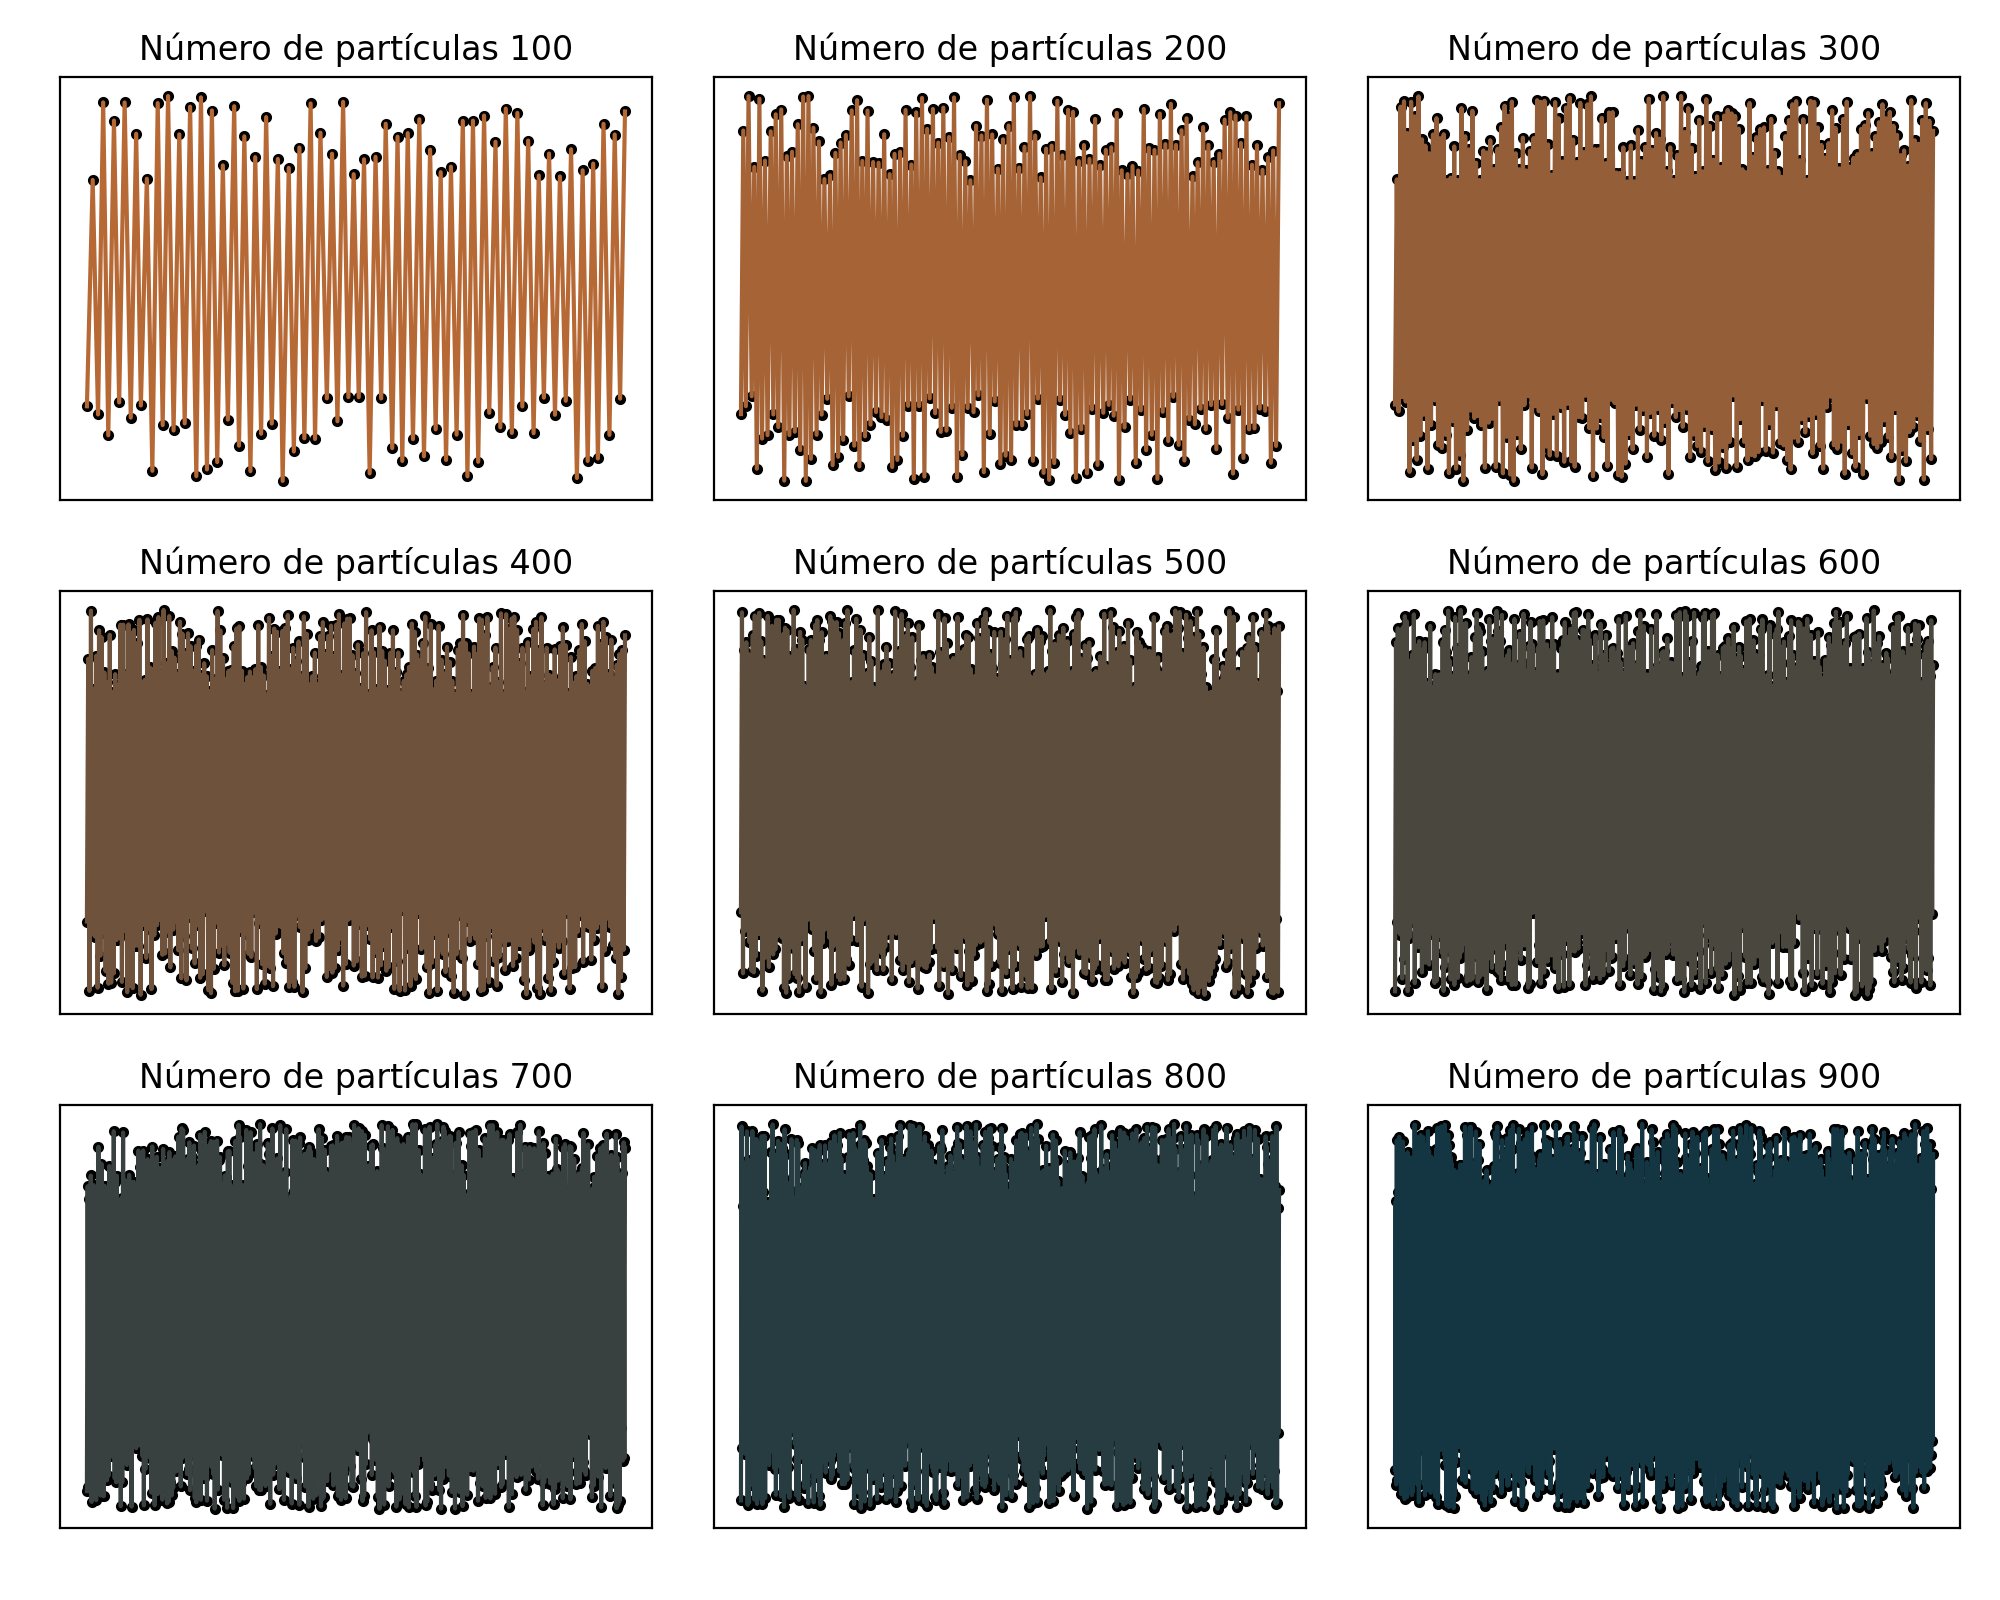
\includegraphics[scale=0.27]{../Graphics/pos_ini.png}
    \caption{Configuración inicial de las cadenas de átomos en cada simulación.}
    \label{fig:posini}
\end{figure}
Las velocidades de cada molecula fueron dada siguiendo las siguientes ecuaciones:
\begin{align*}
    v_{xi}&=v_{0}\cos(2v_0\pi)\\
    v_{yi}&=v_{0}\sin(2v_0\pi)\\
\end{align*}
donde $v_0$ es un número aleatorio entre 0 y 1. Los parámetros usados para cada simulación son los que se muestran en la tabla \ref{table:parametros},
la dinámica que presento cada simulación estan guardadas en el siguiente link (\href{https://github.com/giovannilopez9808/Notas_Agosto_2020/tree/master/Simulaciones/Proyecto_4_2/Graphics/simulaciones}{simulaciones.mp4}).
En cada una de ellas se realizó la monitorización de la energía potencial, energía cinética y las posiciones de cada molecula. En la figura \ref{fig:dim}
se visualiza la dinámica de la cadena de 900 átomos.
\begin{figure}[H]
    \centering
    \hspace{-0.5cm}
    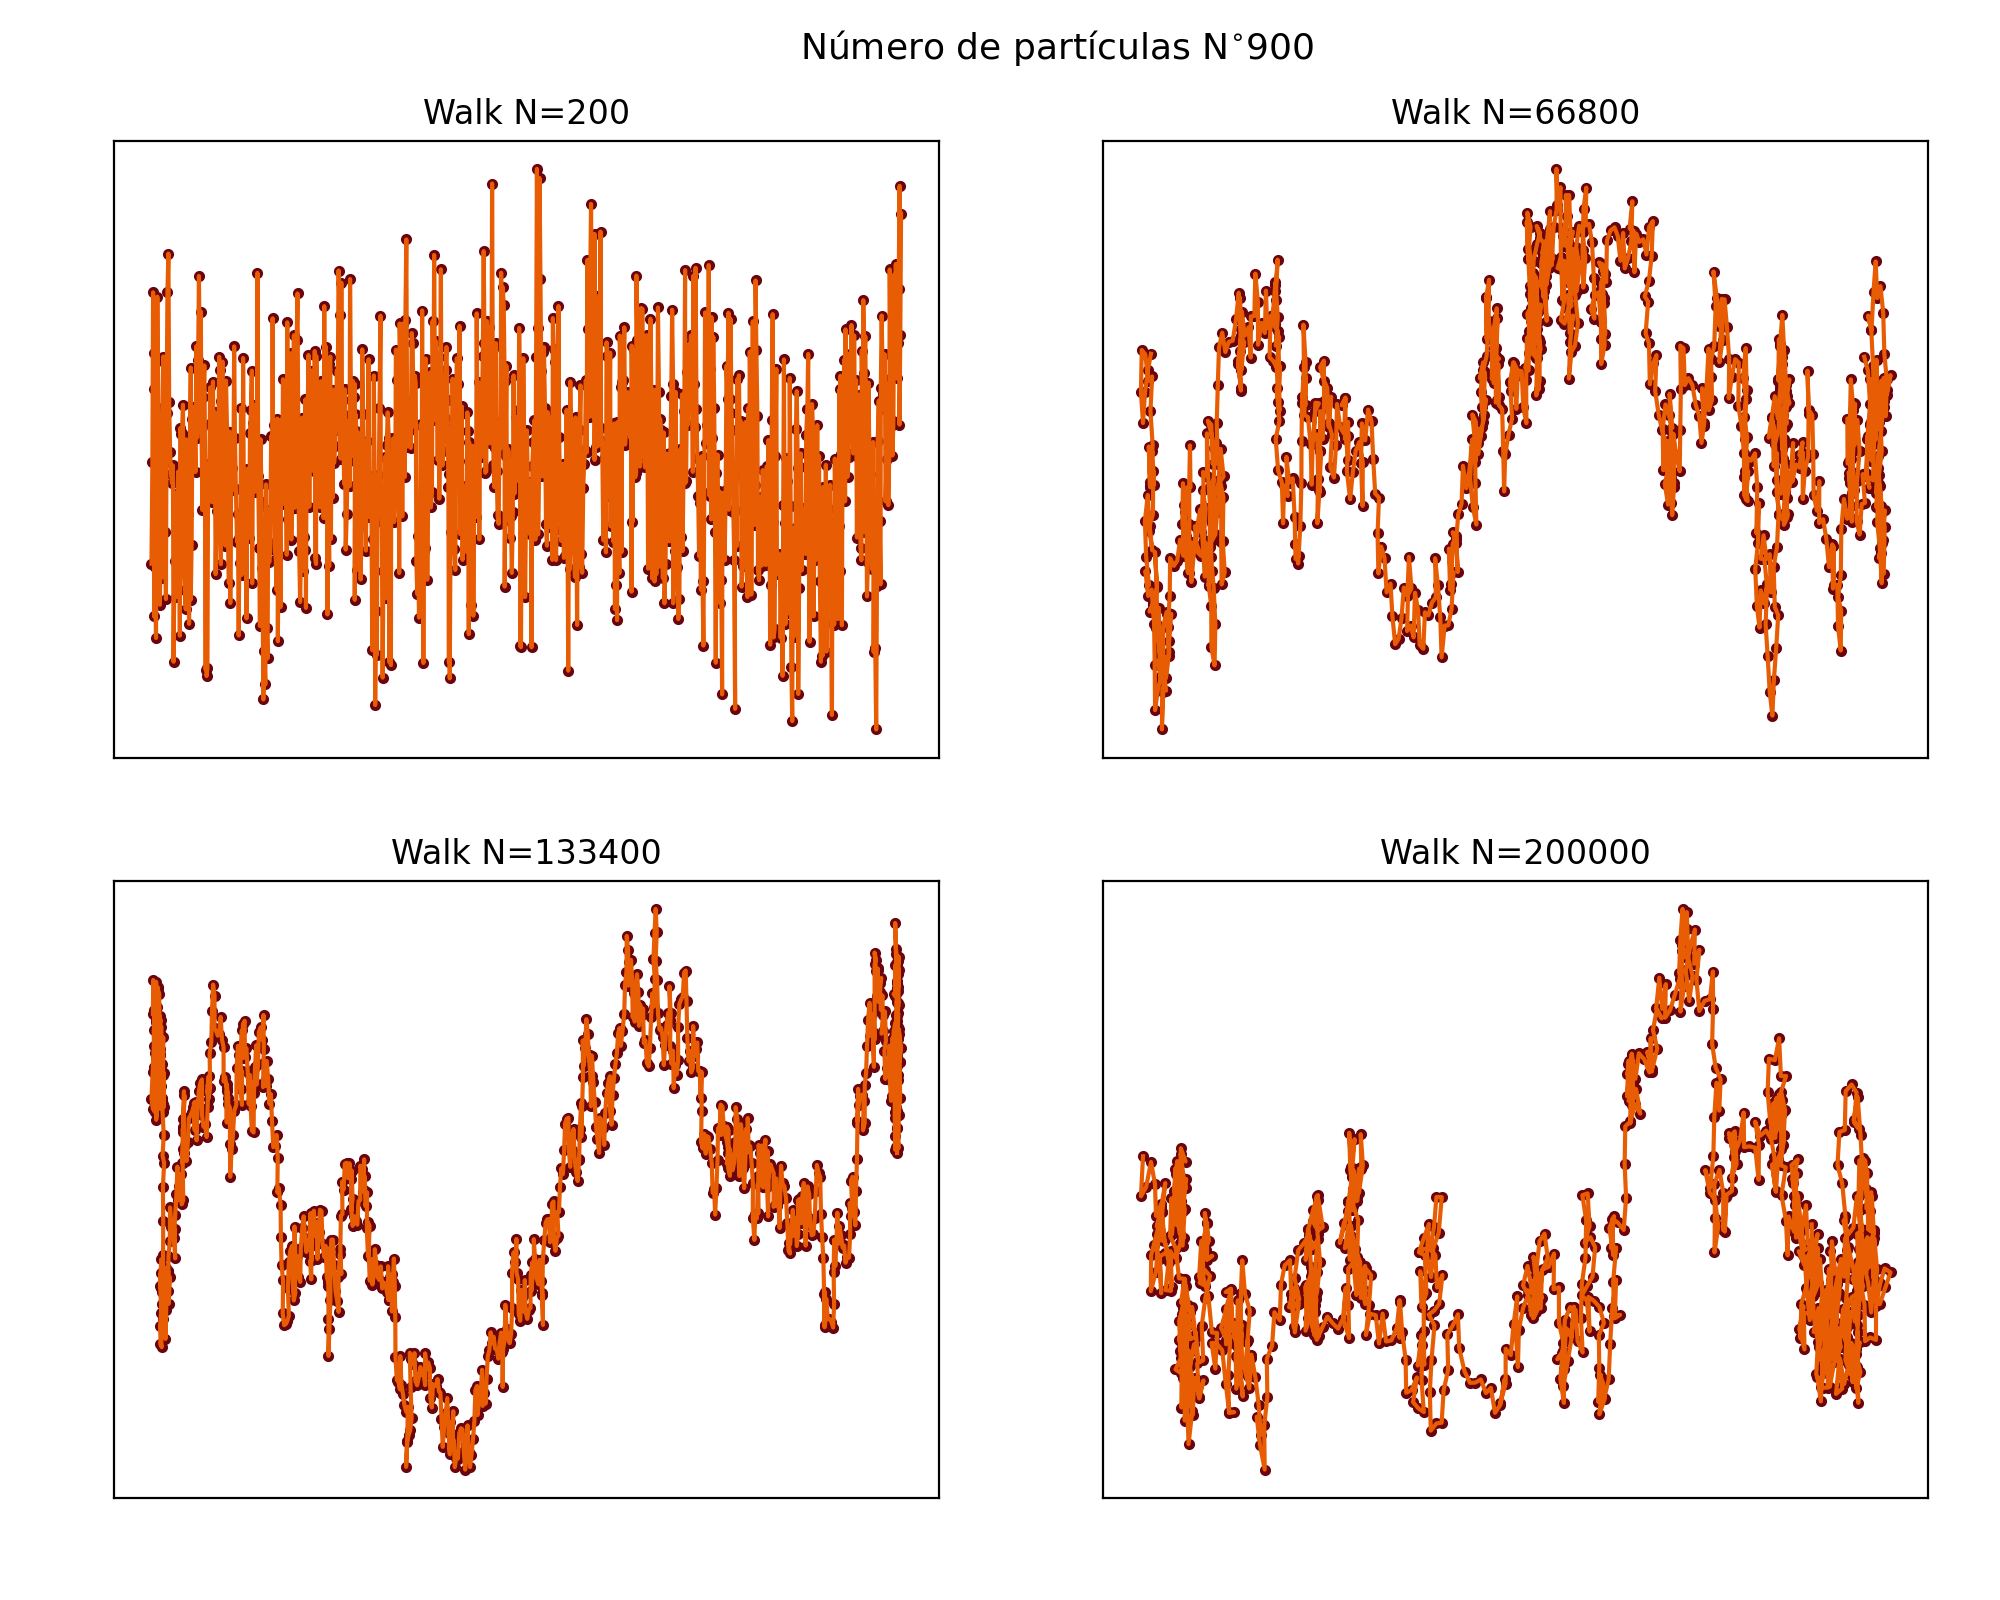
\includegraphics[scale=0.3]{../Graphics/dim_8.png}
    \caption{Dinámica de una simulación de la cadena de 900 átomos a diferentes tiempos.}
    \label{fig:dim}
\end{figure}
\begin{figure}[H]
    \centering
    \hspace{-0.2cm}
    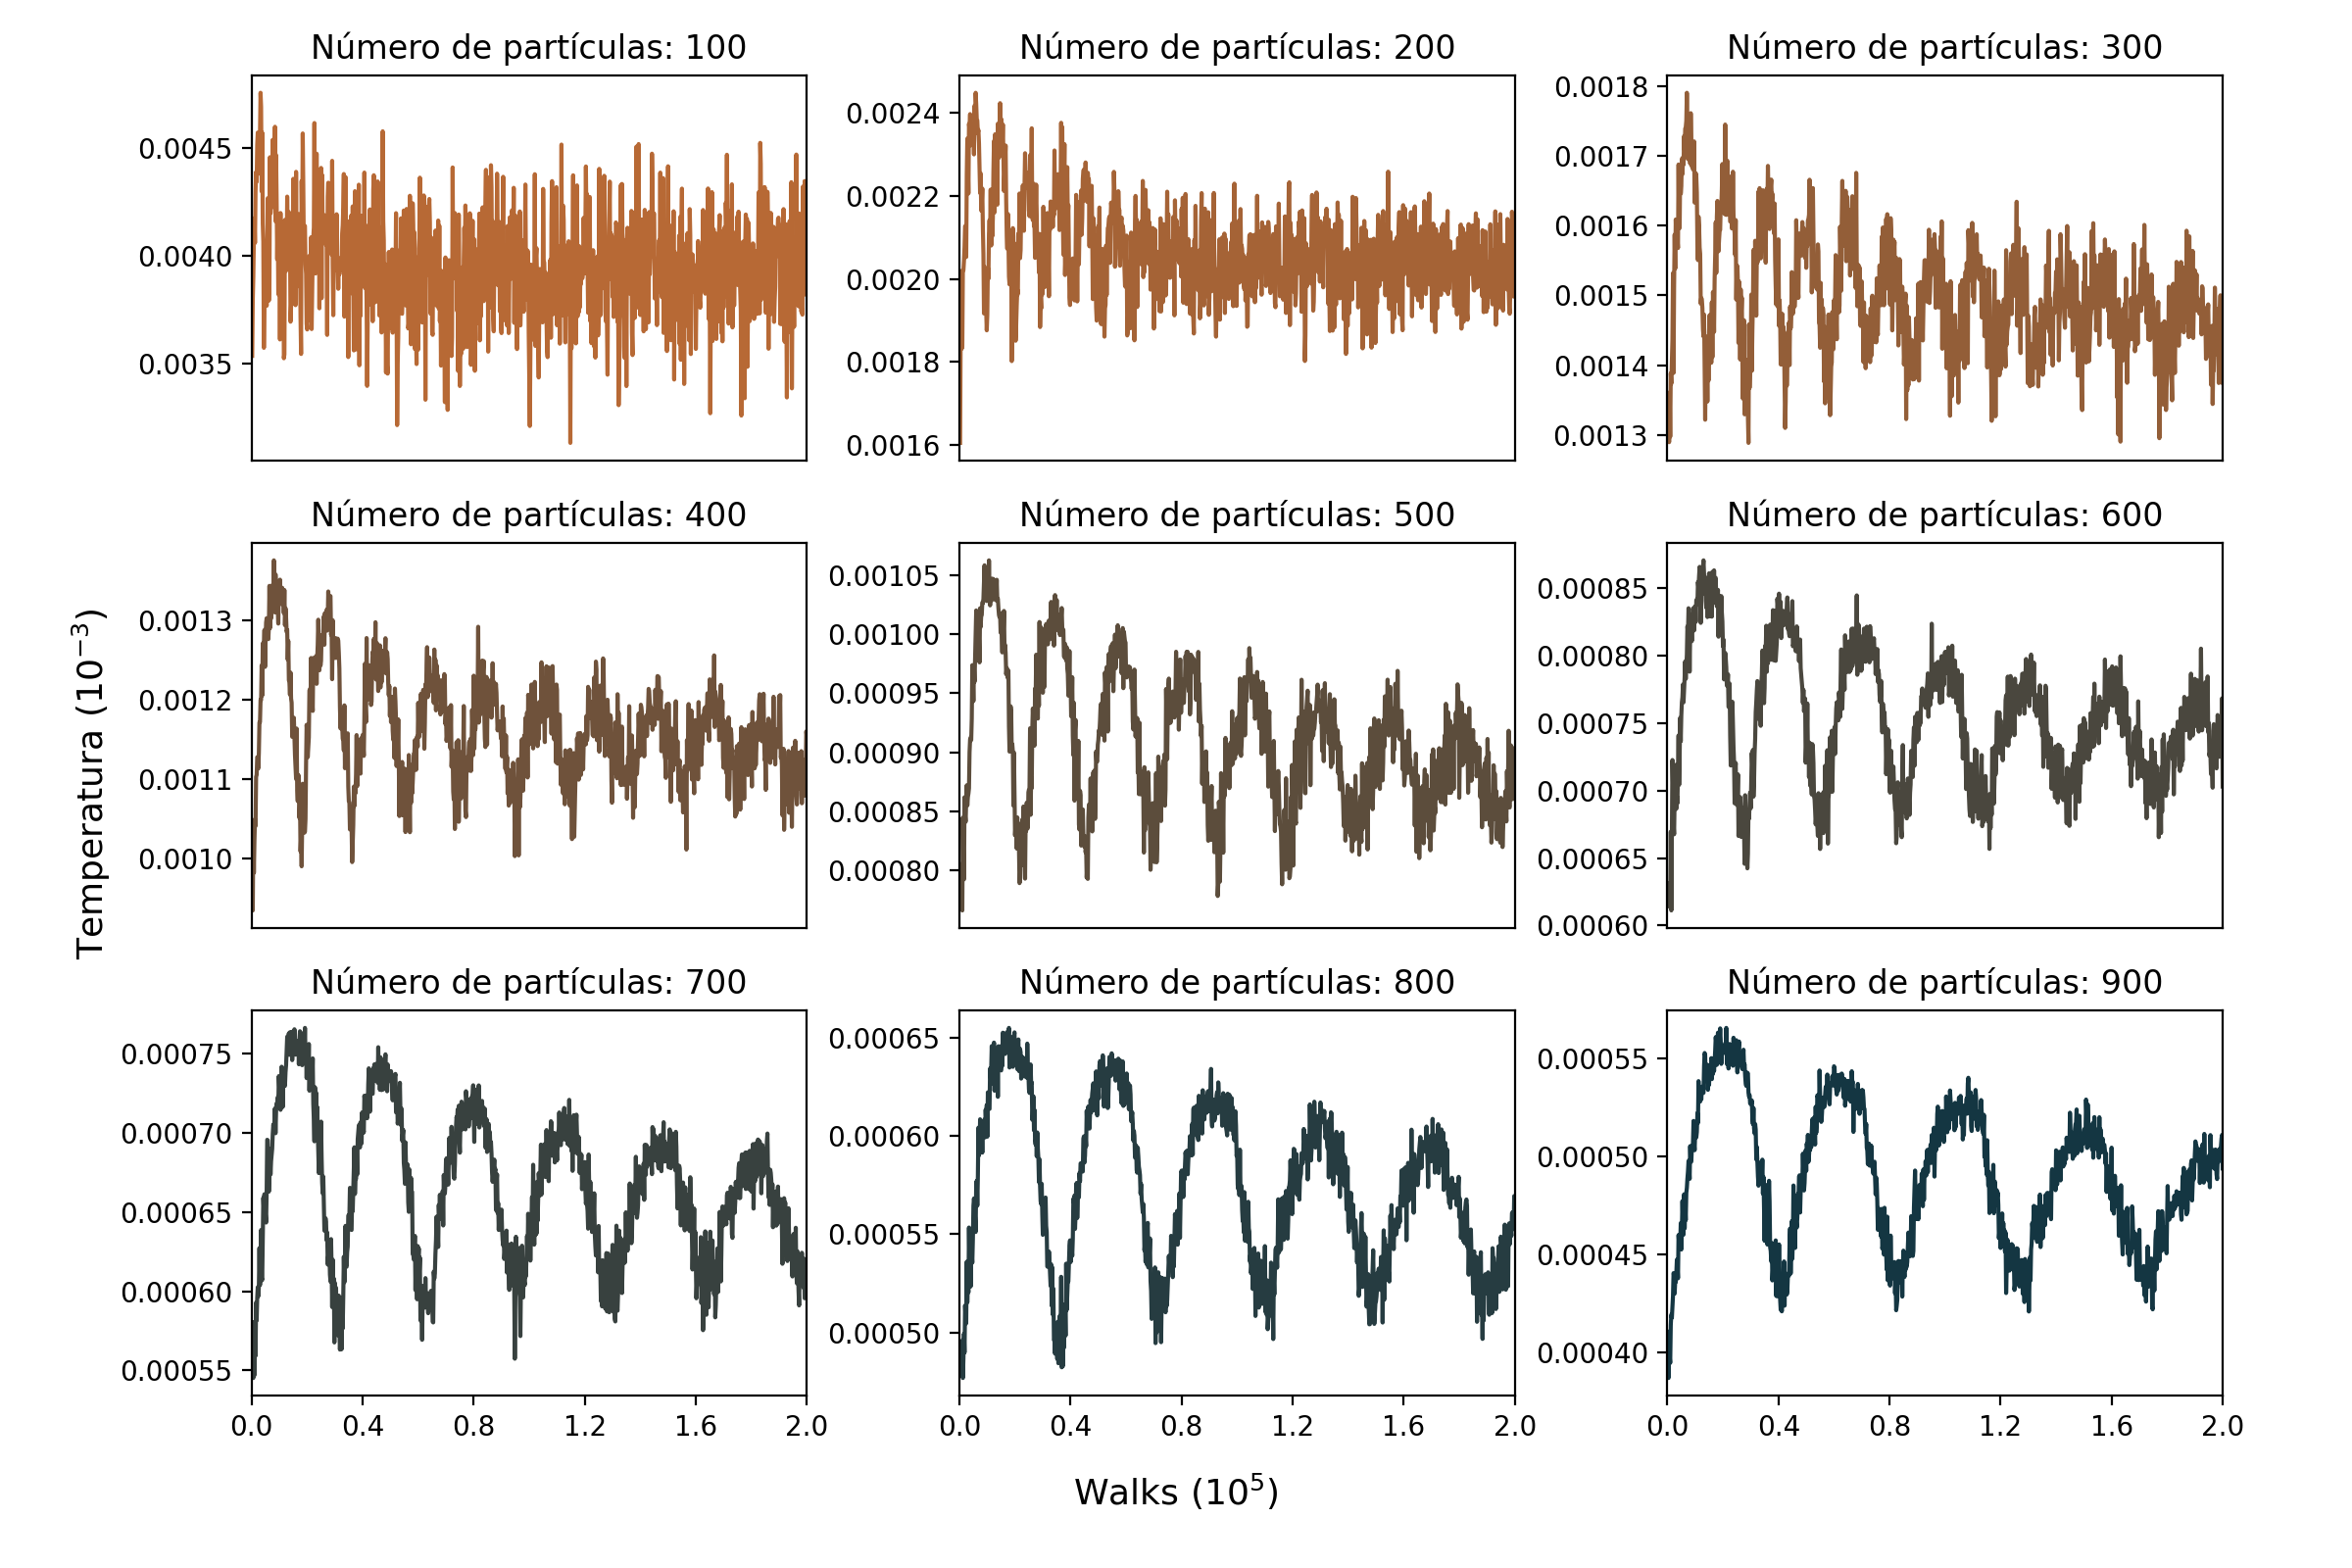
\includegraphics[scale=0.25]{../Graphics/temp.png}
    \caption{Temperatura de las diferentes simulaciones de la cadena de átomos bajo el potencial de Lennard-Jones y el potencual FENE.}
    \label{fig:temp}
\end{figure}
Realizando el calculo de la temperatura del sistema a cada paso de la simulación se obtuvo la figura \ref{fig:temp}.
Observando la variación de la energía potencial a lo largo de la simulación se obtuvo la figura \ref{fig:energy}.
\begin{figure}[H]
    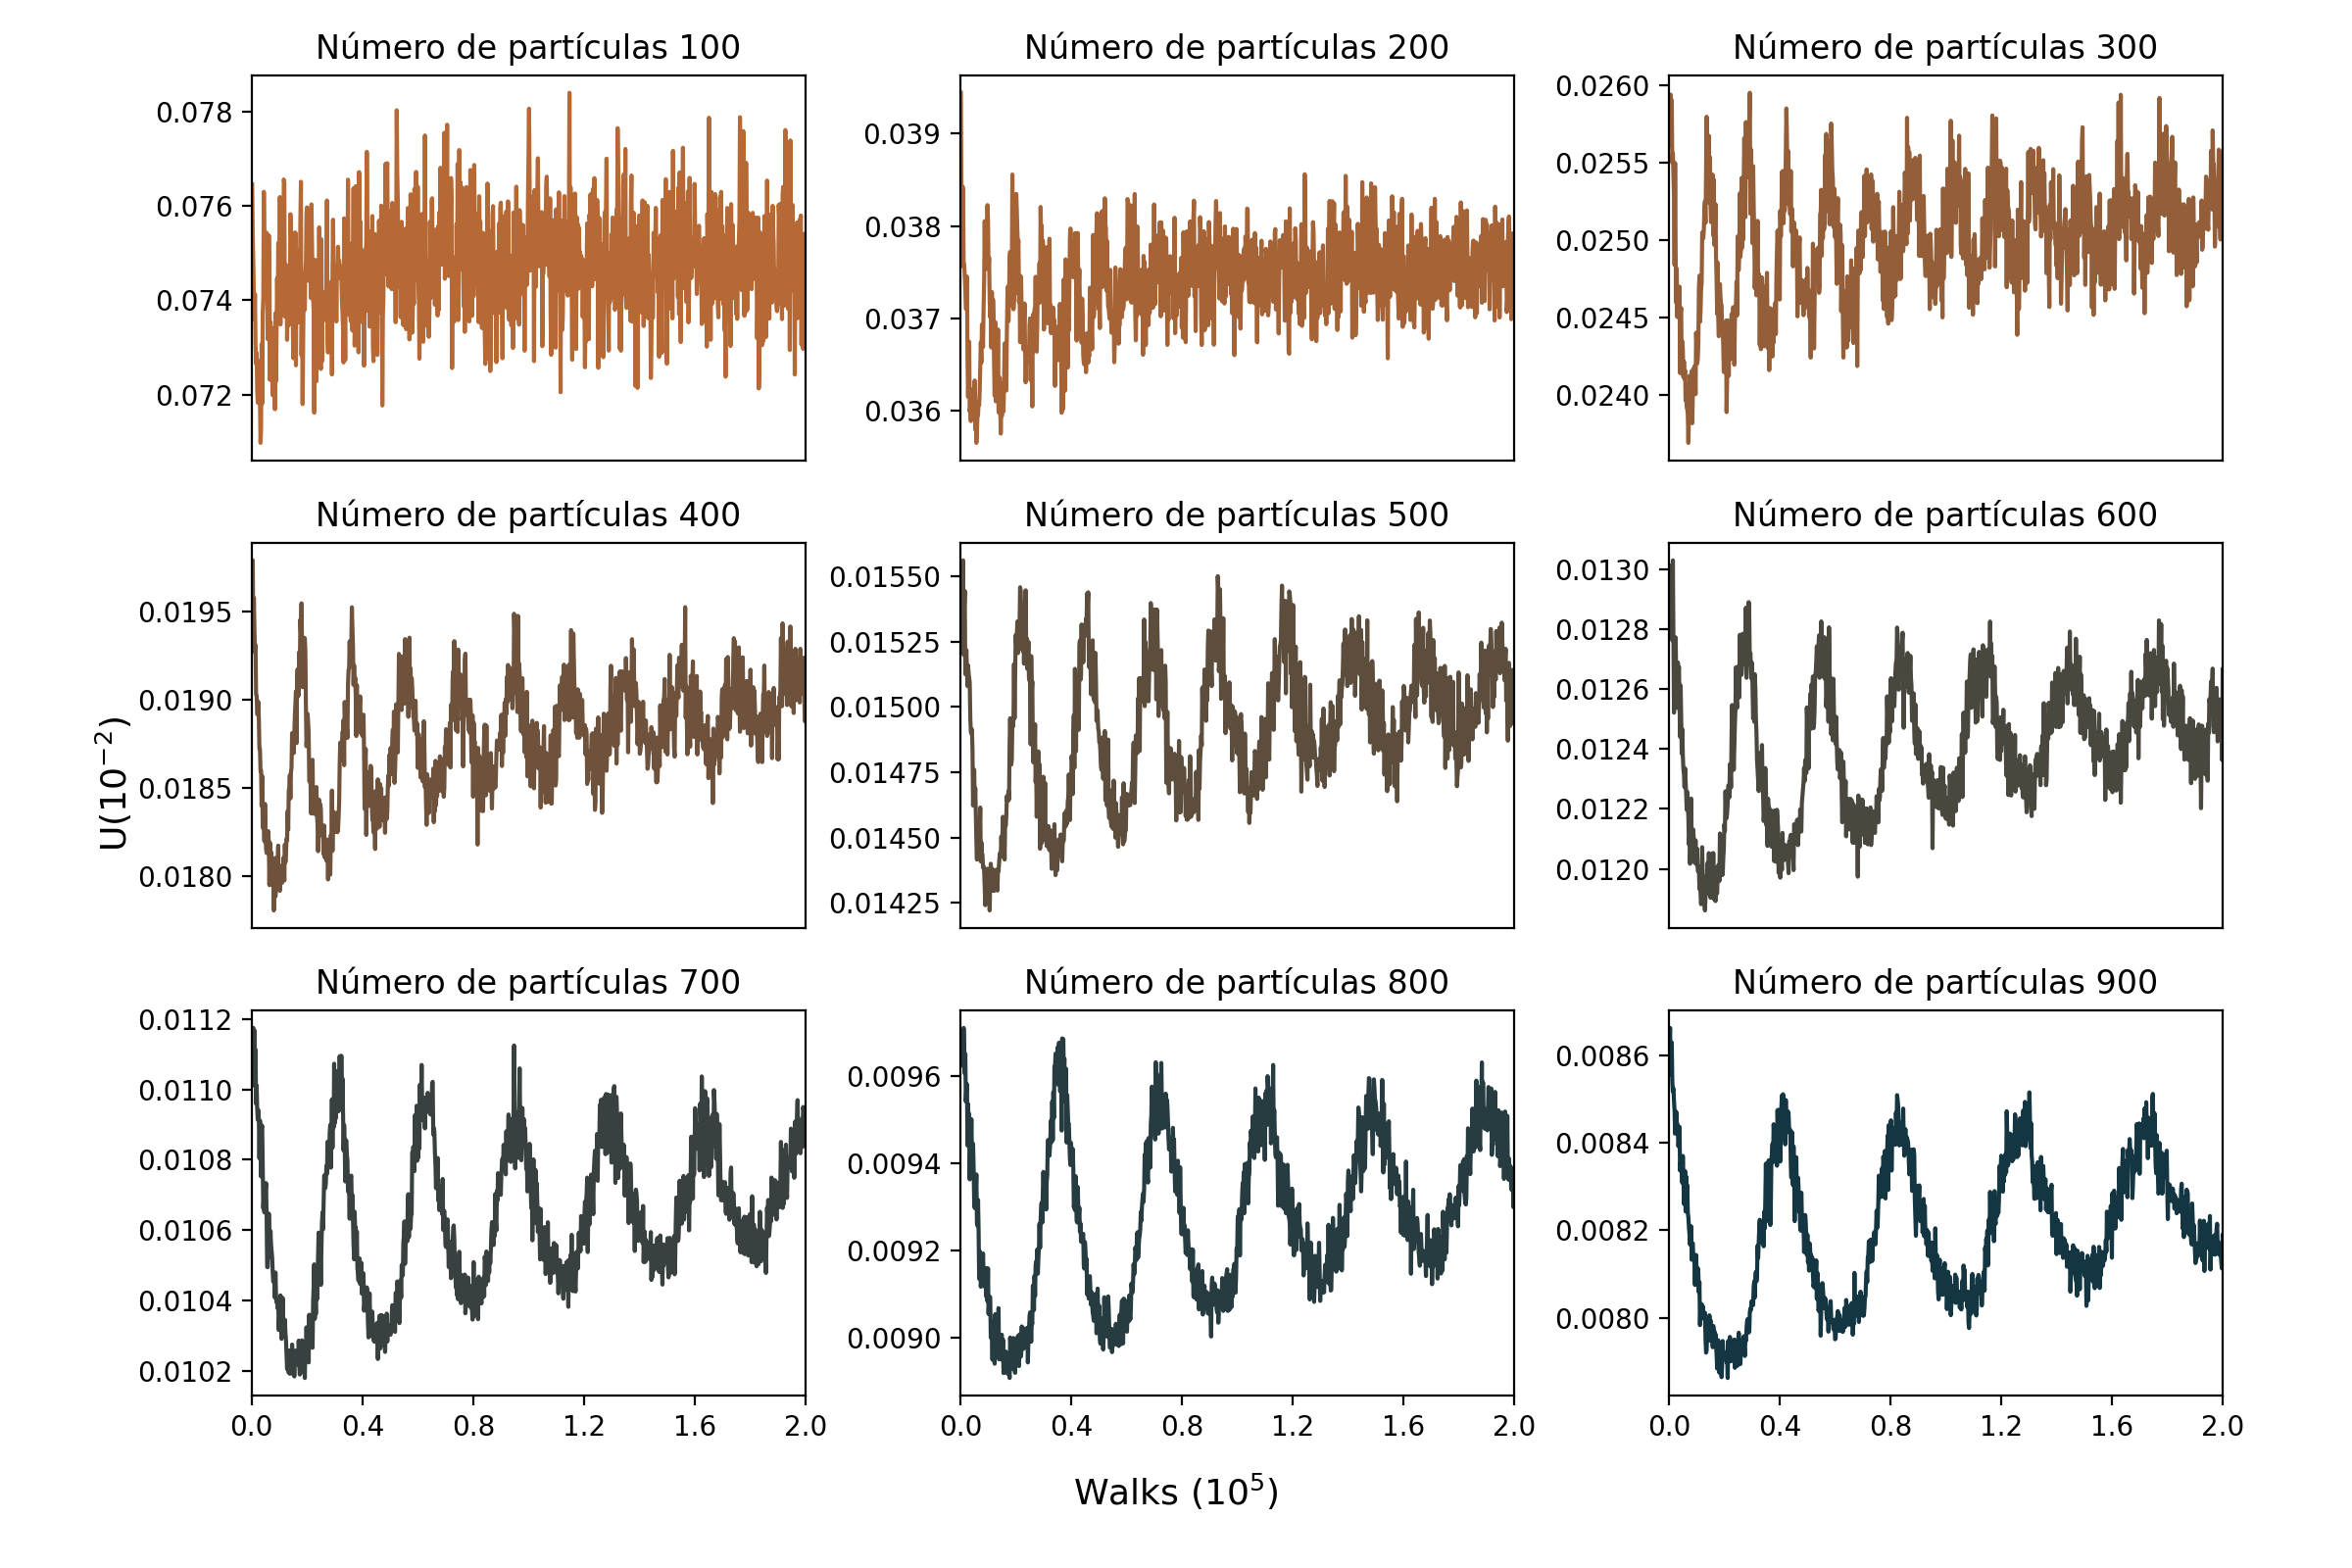
\includegraphics[scale=0.25]{../Graphics/energy.png}
    \caption{Energía potencial de las diferentes simulaciones de la cadena de átomos bajo el potencial de Lennard-Jones y el potencial FENE.}
    \label{fig:energy}
\end{figure}
Obteniendo la distancia entre el primer átomo y último átomo de la cadena de monomeros para cada cierta cantidad de pasos, llamando a esto
como distancia inicio fin, en nuestro caso esta información era calculada
cada 500 pasos, por lo que se obtuvo un valor promedio, estos valores son mostrados en la figura \ref{eq:dis}
\begin{figure}[H]
    \centering
    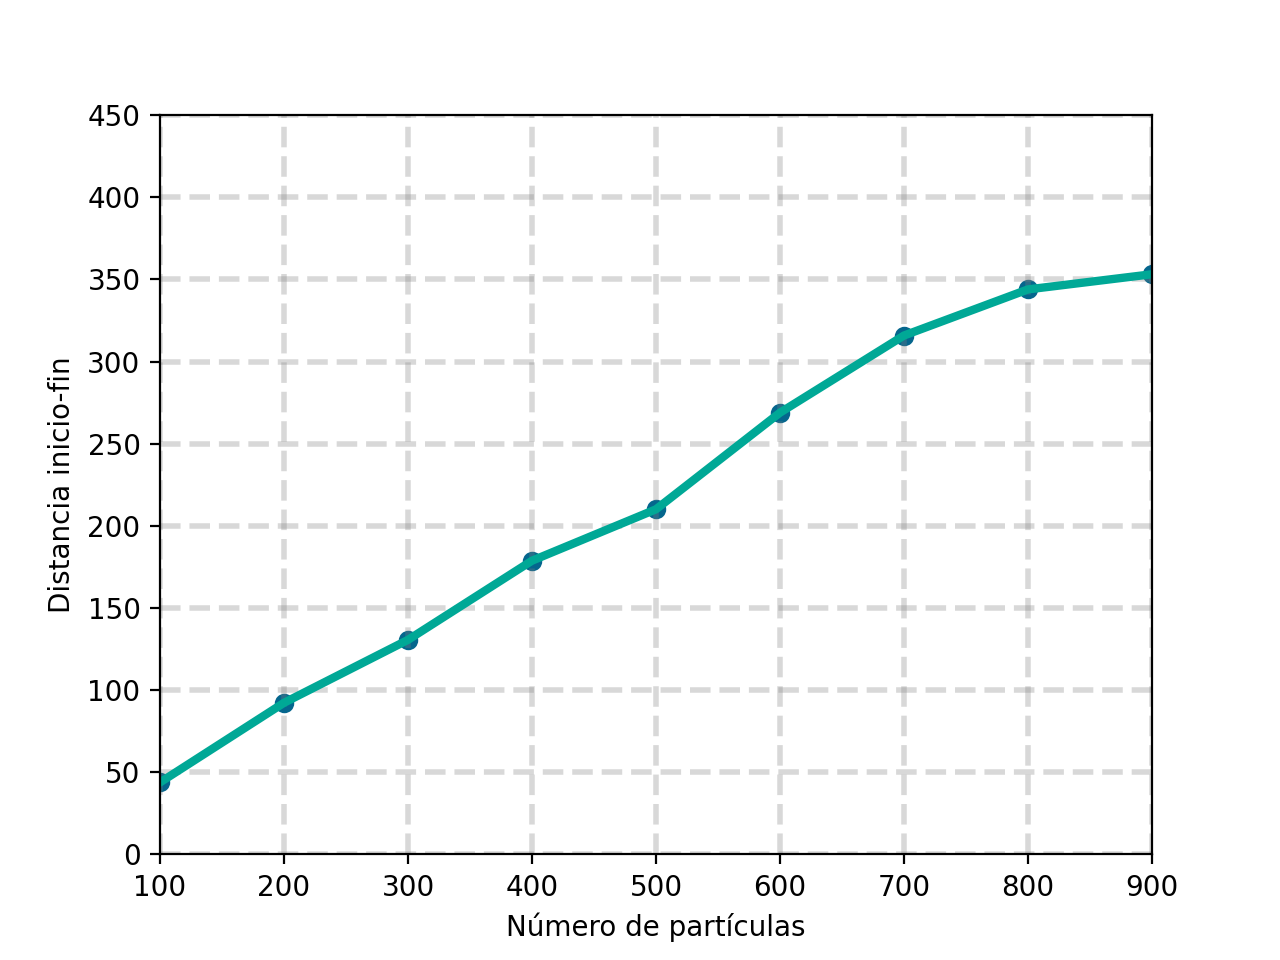
\includegraphics[scale=0.5]{../Graphics/dis.png}
    \caption{Promedios de la distancia inicio fin de cada simulación realizada.}
    \label{eq:dis}
\end{figure}